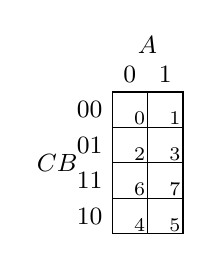
\begin{tikzpicture}[font=\fontsize{9}{10}\selectfont,x=4.5mm,y=4.5mm,baseline=(current bounding box.center)]
\draw (0,0) rectangle (2,4) (1,0)--(1,4);
\foreach \y in {1,2,3}{\draw (0,\y)--(2,\y);}
\node[above] at (1,4.8) {\(A\)};
\node[above] at (.5,4) {0};\node[above] at (1.5,4) {1};
\node[left] at (-.7,2) {\(CB\)};
\foreach \y/\lab in {3.5/00,2.5/01,1.5/11,.5/10}{\node[left] at (0,\y) {\lab};}
\foreach \x/\y/\lab in {1/3/0,2/3/1,1/2/2,2/2/3,1/1/6,2/1/7,1/0/4,2/0/5}{
 \node[anchor=south east,inner sep=.7pt,font=\fontsize{7}{8}\selectfont] at (\x,\y) {\lab};
}
\end{tikzpicture}
